\documentclass[]{beamer}
\usepackage{amsmath}
\usepackage{tikz}
\usepackage{eurosym}

\title[Pratica 2]{Aula Pratica 2}
\author[P. Fagandini]{Paulo Fagandini}
\institute[ISCAL-IPL]{Lisbon Accounting and Business School}
\date{}

\begin{document}

\maketitle

\frame{
O Miguel tem uma mesada de \euro 120 que pode usar para o consumo mensal de bolos e
maçãs. Assuma que um bolo ($x$) custa \euro 2 e uma maçã ($y$) \euro 1 e que as suas preferências
podem ser descritas pela função utilidade $U=\sqrt{xy}$.
}


\frame{
a) Determine analiticamente a restrição orçamental do Miguel e faça a
representação gráfica do espaço das possibilidades de consumo.

\begin{columns}

    \begin{column}{0.49\textwidth}
        \[2 x+1 y=120\]\[y = \frac{120}{1}-\frac{2}{1}x\]\[y = 120-2x\]
    \end{column}

    \begin{column}{0.49\textwidth}
        \begin{figure}
            \centering

            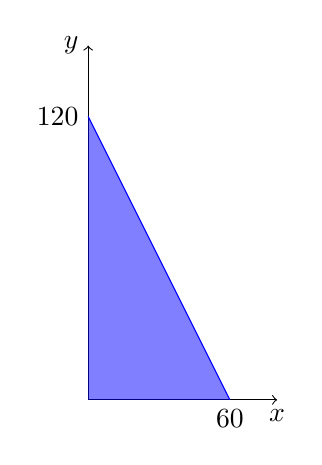
\begin{tikzpicture}[scale = 0.03]

                \onslide<2->{\draw[<->] (0,150) node[left]{$y$} -- (0,0) -- (80,0)node[below]{$x$};}

                \onslide<3->{\draw[blue, domain = 0:60] plot (\x, {120-2*\x});}
                \onslide<4->{
                    \fill[blue, domain=0:60, variable = \x, opacity = 0.5] (0,0) -- plot (\x, {120-2*\x}) -- (0,0) -- cycle;

                    \draw(0, 120) node[left]{$120$};
                    \draw(60,0) node[below]{$60$};
                }

            \end{tikzpicture}
        \end{figure}
    \end{column}
\end{columns}
}

\frame{
b) Represente no gráfico anterior o efeito de uma diminuição do preço dos bolos
para \euro 1.5 na restrição orçamental. Em quanto aumentou a quantidade máxima
que o Miguel pode comprar de bolos? E de maçãs?

\begin{figure}
    \centering

    \begin{tikzpicture}[scale = 0.03]

        \onslide<2->{\draw[<->] (0,150) node[left]{$y$} -- (0,0) -- (100,0)node[below]{$x$};}

        \onslide<3>{
            \draw[blue, domain = 0:60] plot (\x, {120-2*\x});
            \draw(0, 120) node[left]{$120$};
            \draw(60,0) node[below]{$60$};
            }

        \onslide<4->{
            \draw[blue!20, domain = 0:60] plot (\x, {120-2*\x});
            \draw[blue, domain=0:80, variable = \x] plot (\x, {120-1.5*\x});

            \draw(0, 120) node[left]{$120$};
            \draw(80,0) node[below]{$80$};
        }

    \end{tikzpicture}
\end{figure}


}

\frame{
c) Sabemos que o Miguel pode consumir um cabaz com 20 bolos e outro cabaz
com 30 bolos aos novos preços. Quantas maçãs está o Miguel a consumir em
cada um destes cabazes se ambos esgotarem o rendimento do Miguel? Será que
são indiferentes? Quantas maçãs teriam os cabazes se fossem indiferentes? Neste
caso ambos poderiam esgotar o orçamento?

\vspace{1.5em}

\begin{columns}
    \begin{column}{0.49\textwidth}
        \onslide<2->{Cabaz 1:}

        \onslide<3->{\[1.5\times 20 + 1 \times y = 120\]}

        \onslide<4->{\[y = 90\]}

        \onslide<5->{\[u(20,90)=\sqrt{20\times 90} \approx 42.43\]}
    \end{column}

    \begin{column}{0.49\textwidth}
        \onslide<2->{Cabaz 2:}

        \onslide<3->{\[1.5\times 30 + 1 \times y = 120\]}

        \onslide<4->{\[y = 75\]}

        \onslide<5->{\[u(30,75)=\sqrt{30\times 75} \approx 47.43\]}
    \end{column}
\end{columns}
}

\frame{
    \[\sqrt{30\times y} = 42.43\ \Rightarrow\ y = \frac{42.43^2}{30}=60  \]
}

\frame{
d) Calcule a taxa marginal de substituição entre os cabazes da alínea c) e interprete
o seu significado.

\onslide<2->{TMS $\rightarrow$} \onslide<3->{mesmo n\'ivel de utilidade.}

\onslide<4->{Cabaz 1: $(20, 90)$ Cabaz 2: $(30, 60)$}

\onslide<5->{\[\frac{\Delta y}{\Delta x} =} \onslide<6->{\frac{60 - 90}{30 - 20}} \onslide<7->{= \frac{30}{10}=3\]}

}

\frame{
e) Derive a taxa marginal de substituição (TMS) a partir da função utilidade
apresentada. Qual o valor da TMS no cabaz $(x, y) = (40,40)$? Será que se trata
do cabaz de escolha óptima? Justifique.

\onslide<2->{$|TMS|=\frac{umg_x}{umg_y}$}\\
\onslide<3->{$umg_x= u'_x = \left[\sqrt{xy}\right]'_x = \frac{\sqrt{y}}{2\sqrt{x}}$}\\
\onslide<4->{$umg_y= u'_y = \left[\sqrt{xy}\right]'_y = \frac{\sqrt{x}}{2\sqrt{y}}$}\\
\onslide<5->{\(|TMS|=\frac{\frac{\sqrt{y}}{2\sqrt{x}}}{\frac{\sqrt{x}}{2\sqrt{y}}}} \onslide<6->{=\frac{y}{x}\)}

}

\frame{
f) Recorrendo à 2\textsuperscript{a} Lei de Gossen, determine o cabaz de escolha óptima aos preços
iniciais.

\onslide<2->{2\textsuperscript{a} Lei de Gossen: $|TMS|=\frac{p_x}{p_y}$}\\
\onslide<3->{$\frac{y}{x}=\frac{2}{1}$} \onslide<4->{$\Rightarrow} \onslide<5->{\ y = 2x$}\\
\onslide<5->{Restri\c c\~ao or\c camental: $2x + y = 120$}\\
\onslide<6->{$2x + 2x = 120$} or $x = 30$ and $y = 60$.
}

\frame{
g) Dê um exemplo de um cabaz indiferente ao óptimo. Será que pode pertencer ao
espaço das possibilidades de consumo? Justifique.

\onslide<2->{Se $(30, 60)$ \'e o cabaz, \'otimo, a utilidade associada \'e $\sqrt{30\times 60} = 30\sqrt{2}$}\\
\onslide<3->{Se $(\tilde{x}, \tilde{y})$ for indiferente ao \'otimo, $\sqrt{\tilde{x}\tilde{y}}=30\sqrt{2}$}\\
\onslide<4->{Pelo que $\tilde{y}=\frac{1800}{\tilde{x}}$}\\
\onslide<5->{Seja $\tilde{x}=18$, ent\~ao} \onslide<6->{$\tilde{y}=100$ por exemplo.}\\
\onslide<6->{A despesa associada \`a $(18, 100)$ \'e $2\times 18+100\times 1 = 136$} \onslide<7->{maior do que o or\c camento dispon\'ivel de \euro 120.}

}

\frame{
h) Determine a equação que descreve a curva de indiferença que contém o cabaz de
escolha óptima.


\vspace{1em}


\onslide<2->{J\'a fizemos... $\tilde{y}=\frac{1800}{\tilde{x}}$}

}


\frame{

i.0) Encontre a procura pelo bem $x$:

\onslide<2->{Para isso, temos de resolver o problema, mas com $p_x = p_x$}

\onslide<3->{Lembrar, RO $2 x + 1 y = 120$, e 2\textsuperscript{a} L.G. $\frac{y}{x}=\frac{2}{1}$ ou $y = 2 x$}

    \begin{align*}
        \onslide<4->{p_x x + 1\times y = 120 &\wedge y = p_x x} \\
        \onslide<5->{p_x x + p_x x &= 120}\\
        \onslide<6->{2p_x x &= 120}\\
        \onslide<7->{x &= \frac{120}{2p_x} = \frac{60}{p_x}}
    \end{align*}
}


\frame{
i.1) Se o preço dos bolos aumentar para \euro 2.5, o que espera que aconteça à
quantidade consumida deste bem?

\onslide<2->{Pela lei da procura, ira cair. At\'e quanto? Basta substituir na procura:}
\onslide<3->{\(x_2 = \frac{60}{2.5} = 24\)}

}

\frame{
i.2) Aos pre\c cos iniciais, e se a procura for $x = 36-3p_x$ qual o excedente do consumidor pelo consumo de $x$?

\onslide<2->{$p_x = 2$, $x=30$}

\begin{figure}
    \centering
    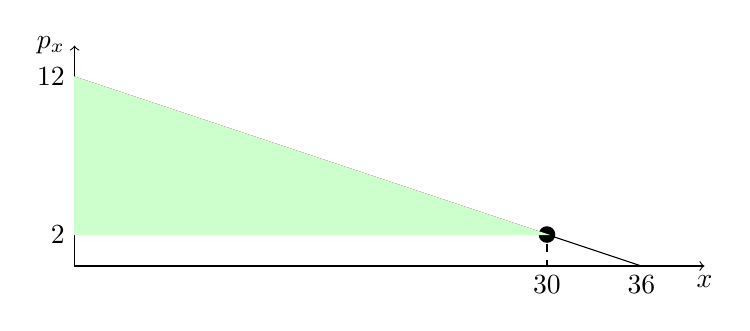
\begin{tikzpicture}[scale = 0.2]
        \onslide<3->{\draw[<->] (0, 14)node[left]{$p_x$} -- (0,0) -- (40, 0)node[below]{$x$};}
        \onslide<4->{
            \draw[domain=0:36] plot (\x, {12-\x/3});
            \draw (0,12) node[left]{$12$};
            \draw (36,0) node[below]{$36$};
        }
        \onslide<5->{
            \draw[dashed] (0,2) node[left]{$2$} -- (30, 2) -- (30, 0)node[below]{$30$};
            \fill (30, 2) circle (15pt);
        }

        \onslide<6->{
            \draw[fill, green!20] (0,2) -- (0,12) -- (30,2) -- (0,2)--cycle;
        }
    \end{tikzpicture}
\end{figure}

\onslide<7->{
    \[X_D=\frac{(12-2)\times(30-0)}{2}=\frac{10\times 30}{2} = \frac{300}{2}=150\]
}

}

\end{document}
